\documentclass{beamer}
\usepackage{etex}
\usepackage{lmodern}
\usepackage[english]{babel}
\usepackage[T1]{fontenc}
\usepackage[utf8]{inputenc}
\usepackage{pst-sigsys} 
\usepackage{amsmath,amsfonts,amssymb}
\usepackage{pstricks-add} 
\usepackage{ragged2e}
\usepackage{graphicx}
\usepackage{ulem}
\usepackage{fontawesome}
\setbeamertemplate{navigation symbols}{}  
 
\usetheme{Darmstadt}
\setbeamertemplate{footline}{\insertframenumber/\inserttotalframenumber}
\title{M1 IEAP - BTI/FH/IEMH\\pFIEA02CM : Analyse et Traitement du Signal}
\author{Flavy ROSEREN\\Martin EGIZIANO\\Frank BULOUP}
\institute{Aix Marseille Université\\Institut des Sciences du Mouvement}
\date{}

\setbeamertemplate{footline} 
{  
	\begin{beamercolorbox}[ht=2.5ex,dp=1.125ex,%
      leftskip=.3cm,rightskip=.3cm plus1fil]{title in head/foot}%
      {\usebeamerfont{title in head/foot}\insertshorttitle} \hfill    
      \insertframenumber / \inserttotalframenumber%
    \end{beamercolorbox}%
%     \begin{beamercolorbox}[colsep=1.5pt]{lower separation line foot}
%     \end{beamercolorbox} 
}

\newcounter{exampleBlockCounter}
\setcounter{exampleBlockCounter}{1}

\begin{document} 
 
\begin{frame}[plain] 
	\titlepage 
	\center{\includegraphics[scale=0.75]{images/by-nc-sa.eps}}
	\vspace{1cm}
	
\includegraphics[scale=0.6]{images/LogoAMU.png}\hspace*{2cm}
	\includegraphics[scale=0.2]{images/LogoCNRS.eps}\hspace*{2cm}
	
\includegraphics[scale=0.1]{images/LogoISM.eps}
\end{frame}

\begin{frame}{Deuxième Partie}
	\tableofcontents
\end{frame}

\section{Transformée en z et filtrage numérique}
\subsection{Exemples de traitements mathématiques}

\begin{frame}
\begin{block}{Calcul numérique}
\justify La plupart des traitements mathématiques peuvent être réalisés en
calcul numérique sur ordinateur :
\begin{itemize}
  \item Moyenne
  \item Dérivée
  \item Lissage
\end{itemize}
\end{block}
\pause
\begin{block}{Filtre numérique}
Ces traitements peuvent être représentés par un filtre numérique
\begin{itemize}
  \item Moyenne $\Leftrightarrow$ filtre moyenneur $\Leftrightarrow$
  \textbf{filtre passe-bas}
  \item Dérivée $\Leftrightarrow$ filtre dérivateur $\Leftrightarrow$
  \textbf{filtre passe-haut}
  \item Lissage $\Leftrightarrow$ généralisation du \textbf{filtre passe-bas}
\end{itemize}
\center
\alert{Filtre passe-bande = filtre passe-bas + filtre passe-haut}
\end{block}
\end{frame}

\begin{frame}
\begin{block}{Moyenne}
\justify Moyenne sur $N$ points :
$$
s(n) = \frac{1}{N}\sum_{k=0}^{N-1}e(n-k)
$$
Sur quatre points :
$$
s(n) = \frac{e(n) + e(n-1) + e(n-2) + e(n-3)}{4}
$$
\end{block}
\pause
\begin{block}{Dérivée}
Le signal a été échantillonné à la fréquence $F_e$ :
$$
s(n) = \frac{e(n) - e(n-1)}{Te}
$$
\end{block}
\end{frame}

\begin{frame}{Généralisation}
\begin{block}{Filtres non récursifs}
\justify Les échantillons passés de la sortie ne sont pas réemployés dans les
calculs :
$$
s(n)=\sum_{k=0}^{N-1}b(k)e(n-k)
$$
\end{block}
\pause
\begin{block}{Filtres récursifs}
\justify Des échantillons passés de la sortie sont mémorisés et réemployés dans
les calculs :
$$
s(n)=\sum_{k=0}^{N-1}b(k)e(n-k) - \sum_{k=0}^{M-1}a(k)s(n-k)
$$ 
\end{block}
\end{frame}

\subsection{Transformée en $z$ : l'opérateur $z^{-1}$}

\begin{frame}
\justify Représenter un filtre numérique sous la forme d'une équation de
récurrence n'est pas la seule possibilité. En passant de l'espace temporel à
l'espace fréquenciel par transformée de Fourier, on obtient une autre
représentation qui fait apparaître l'opérateur de retard, noté $z^{-1}$. Cet
opérateur, appliqué à un signal $s(n)$, le retarde d'un échantillon.
\pause
\begin{block}{Transformée en $z$}
\justify La transformée en $z$ découle directement de la TFD (Cf. séquence $5$).
En posant $z=e^{2i\pi\frac{k}{N}}$ dans l'expression de la TFD, on obtient :
$$
S(z) = \sum_{k=0}^{N-1}s(k)z^{-k}
$$
\end{block}
\end{frame}

\begin{frame}
\begin{exampleblock}{Exercice sur l'opérateur de retard}
	\justifying
	Calculer les TZ des signaux suivants :
\begin{itemize}
	\item $e(n-1)$
	\item $e(n-2)$
	\item $e(n-3)$
	\item Généraliser pour en déduire le théorème du retard
\end{itemize}	
\end{exampleblock}
\end{frame}

\begin{frame}
\begin{exampleblock}{Exercice sur l'opérateur de retard}
\begin{align*}
TZ\{e(n-1)\} &= z^{-1}E(z)
\end{align*}
\pause
\begin{align*}
TZ\{ e(n-1)\} &= z^{-2}E(z)\\
TZ\{ e(n-3)\} &= z^{-3}E(z)
\end{align*}
\pause
\begin{align*}
TZ\{ e(n-m)\} &= z^{-m}E(z)
\end{align*}
\end{exampleblock}
\end{frame}

\begin{frame}
\begin{exampleblock}{Calcul de Transformée en $z$}
	\justifying
	Calculer les TZ des équations suivantes :
	\itemize
	\item La moyenne : $s(n) = \frac{e(n) + e(n-1) + e(n-2) + e(n-3)}{4}$
	\item La dérivée : $s(n) = \frac{e(n) - e(n-1)}{T_e}$
	\item Un filtre non récursif : $s(n)=\sum_{k=0}^{N-1}b(k)e(n-k)$
	\item Un filtre récursif : $s(n)=\sum_{k=0}^{N-1}b(k)e(n-k) -
	\sum_{k=1}^{M-1}a(k)s(n-k)$
\end{exampleblock}
\end{frame}

\begin{frame}
\begin{exampleblock}{Calcul de Transformée en $z$}
Moyenne :
$$
S(z)=\frac{E(z)+z^{-1}E(z)+z^{-2}E(z)+z^{-3}E(z)}{4}
$$
\pause
Dérivée :
$$
S(z)=\frac{E(z)-z^{-1}E(z)}{T_e}
$$
\end{exampleblock}
\end{frame}

\begin{frame}
\begin{exampleblock}{Calcul de Transformée en $z$}
Filtre non récursif :
$$
S(z)=\sum_{k=0}^{N-1}b(k)z^{-k}E(z)
$$
\pause
Filtre récursif :
$$
S(z)=\sum_{k=0}^{N-1}b(k)z^{-k}E(z) - \sum_{k=1}^{M-1}a(k)z^{-k}S(z)
$$
\end{exampleblock}
\end{frame}


\begin{frame}
\justify
L'utilsation de la transformée en $z$, et donc le passage dans le domaine
fréquenciel, permet de simplifier l'écriture en ne faisant apparaître que
l'opérateur $z^{-1}$. Par exemple :
$$
s(n) = e(n) + e(n-1)
$$
On obtient par TZ :
$$
S(z) = E(z) + z^{-1}E(z) = (1+z^{-1})E(z)
$$
Et on peut alors écrire :
$$
\frac{S(z)}{E(z)} = 1+ z^{-1}
$$
\end{frame}

\subsection{Fonction de Transfert en $z$}

\begin{frame}
\begin{block}{Défintion}
\justify On appelle fonction de transfert en $z$, que l'on note souvent $H(z)$,
le quotient de $S(z)$ par $E(z)$ :
$$
H(z) = \frac{S(z)}{E(z)}
$$ 
\end{block}
\pause
\begin{block}{Remarques}
\begin{itemize}
  \item $H(z)$ est une fraction rationnelle en $z$
  \item On utilise son expression pour créer un filtre sous Python
  \item Il faut la toolbox Signal Processing
  \item On ne saisit alors que les coefficients des polynômes en $z$ du
  dénominateur et du numérateur de $H(z)$
\end{itemize}
\end{block}
\end{frame}

\begin{frame}
\justify Par exemple :
$
H(z) = 1+z^{-1} = \frac{1+z^{-1}}{1} = \frac{b(1) + b(2)z^{-1}}{a(1)}
$
\justify On peut alors en déduire les vecteurs suivants sous Python :
$$
b = [1\text{, }1]\text{ et }a = [1]
$$
\begin{exampleblock}{Calcul de fonction de transfert $H(z)$}
\justify Écrire les fonctions de transfert pour le filtre :
\begin{enumerate}
  \item moyenneur
  \item dérivateur
  \item récursif
  \item non récursif
\end{enumerate}
\justify Donner les vecteurs $a$ et $b$ pour les deux premiers filtres
\end{exampleblock}
\end{frame}

\begin{frame}
\begin{exampleblock}{Calcul de fonction de transfert $H(z)$}
Moyenneur :
$$
H(z) = \frac{1}{4}+\frac{1}{4}z^{-1}+\frac{1}{4}z^{-2}+\frac{1}{4}z^{-3}
$$
\pause
Dérivateur :
$$
H(z) = \frac{1-z^{-1}}{T_e}
$$
\end{exampleblock}
\end{frame}

\begin{frame}
\begin{exampleblock}{Calcul de fonction de transfert $H(z)$}
Filtre non récursif :
$$
H(z) = \sum_{k=0}^{N-1}b(k)z^{-k}
$$
\pause
Filtre récursif :
$$
H(z) = \frac{\sum_{k=0}^{N-1}b(k)z^{-k}}{1+\sum_{k=1}^{M-1}a(k)z^{-k}}
$$
\end{exampleblock}
\end{frame}

\subsection{Les filtres RIF}
\begin{frame}
\begin{block}{Filtre non récursif}
\justify Dit aussi filtre à réponse impulsionnelle finie (RIF)
\center
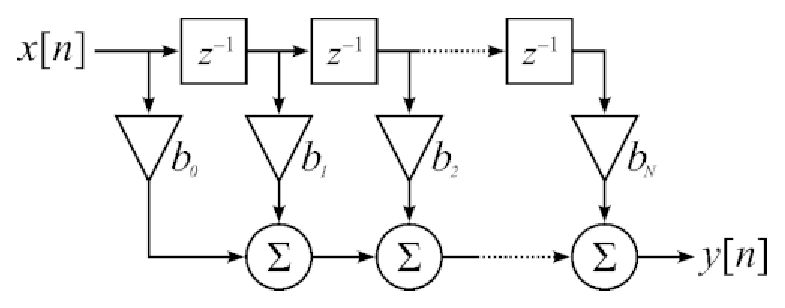
\includegraphics[scale=.6]{images/FiltreRIF-2.eps}
\end{block}
\end{frame}

\begin{frame}
\center
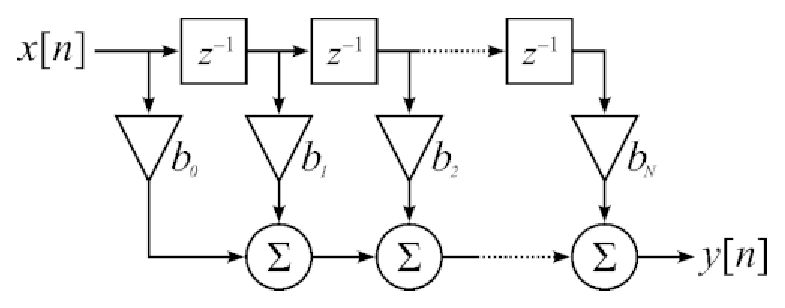
\includegraphics[scale=.6]{images/FiltreRIF-2.eps}
\begin{block}{Propriétés}
\begin{itemize}
  \item Ils sont toujours stables
  \item Ils ne propage pas les erreurs de calculs numériques
  \item Ils sont à phase linéaire (retard uniquement)
  \item Ils sont moins sélectifs que les RII pour un même ordre
\end{itemize}
\end{block}
\end{frame}  

\subsection{Les filtres RII}
\begin{frame}
\begin{block}{Filtre récursif} 
\justify Dit aussi filtre à réponse impulsionnelle infinie (RII)
\center
\includegraphics[scale=.25]{images/FiltreRII.eps}
\end{block}
\end{frame}

\begin{frame}
\center
\includegraphics[scale=.15]{images/FiltreRII.eps}
\begin{block}{Propriétés}
\begin{itemize}
  \item Ils ne sont pas toujours stables (choisir une méthode de synthèse)
  \item Ils faut mémoriser plus d'échantillons passés
  \item Ils propagent les erreurs de calculs
  \item Ils sont à phase non linéaire (déformation du signal)
  \item Ils sont plus sélectifs que les RIF pour un même ordre
\end{itemize}
\end{block}
\end{frame}

\subsection{Exercices Python}
\begin{frame}
\begin{exampleblock}{Exercice I}
Soit le signal suivant $s(t)$ échantillonné à $F_e=4Hz$ :
$$s(t) = 3 + sin(2\pi t)$$ 
\begin{enumerate}
  \item Représenter le signal sur une durée de $10s$
  \item Lire l'aide de la fonction Python \textbf{filter}
  \item Programmer un filtre moyenneur sur $4$ points
  \item Programmer un filtre dérivateur
  \item Comparer la dérivée théorique avec la sortie du dérivateur. Conclusion ?
\end{enumerate}
\end{exampleblock}
\end{frame}

\begin{frame}
\begin{exampleblock}{Exercice II}
\begin{enumerate}
  \item Charger le fichier de la note Mi
  \item Calculer le module de la TFD de ce signal
  \item Tracer le spectre monolatéral. Quelles informations en tirez-vous ?
  \item Ajouter un bruit blanc (voir avec le prof.)
  \item Filtrer avec un filtre de type RII. Utiliser la fonction \textbf{butter}
  \item Proposer un ordre et une fréquence de coupure permettant de supprimer au
  mieux le bruit sans détruire l'information
  \item Filtrer avec un filtre de type RIF. Utiliser la fonction \textbf{firpm}
  \item Proposer un filtre RIF qui soit équivalent au filtre RII précédent
  \item Conclure
\end{enumerate}
\end{exampleblock}
\end{frame}

\end{document}
